\section{Heaps}

\begin{frame}
	\begin{block}{Heap}
		\begin{itemize}
			\item Estrutura de dados em árvore com algumas propriedades específicas:
			\item É uma árvore completa (todos os níveis, com exceção do último tem que ser preenchidos)
			\item Um Heap binário sempre será um Min Heap ou Max Heap.
			\item Um Heap mínimo tem em sua raiz o menor elemento possível do conjunto. Essa propriedade também se aplica as subárvores do heap.
			\item Um Heap máximo tem em sua raiz o maior elemento possível do conjunto. Essa propriedade também se aplica as subárvores do heap.
		\end{itemize}
	\end{block}
\end{frame}

\begin{frame}
	\begin{block}{Heap}
		\begin{figure}[!htb]
			\centering	  				
			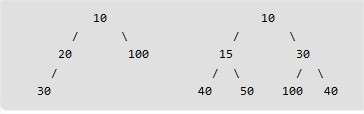
\includegraphics[height=3cm, width = 9cm]{./pic/heap.jpg}
			\caption{Exemplo de Heap}
			\label{fig_pilha}
		\end{figure}
	\end{block}
\end{frame}

\begin{frame}
	\begin{block}{Heap}
		\begin{itemize}
			\item Tipicamente Heap's são representados usando vetores (denominado V para exemplo didático) onde:
			\item  $V[0]$ é a raiz do meu heap
			\item Por estar completo em todos os níveis, exceto o último (não sendo obrigatório o preenchimento deste) satisfaz a seguinte relação:
			\item $V[1/2]$ retorna o nó pai
			\item $V[(2*i)+1]$ retorna o filho da esquerda
			\item $V[(2*i)+2]$ retorna o filho da direita
		\end{itemize}
	\end{block}
\end{frame}

\begin{frame}
	\begin{block}{Heap}
		\begin{figure}[!htb]
			\centering	  				
			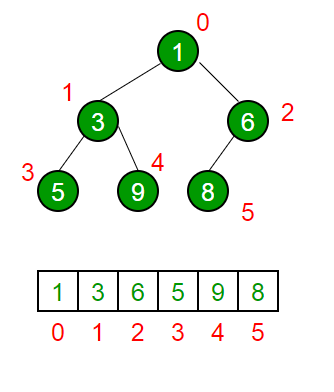
\includegraphics[height=3cm, width = 9cm]{./pic/binaryheap.png}
			\caption{Exemplo de Heap}
			\label{fig_pilha}
		\end{figure}
	\end{block}
\end{frame}


\begin{frame}
	\begin{block}{Heap}
		\begin{itemize}
			\item As árvores Heap tem algumas aplicações na ciência da computação. Podemos citar o algoritmo de ordenação heapSort, filas de prioridade, grafos pois os algoritmos de Dijsktra e Prim usam essas estruturas.
		\end{itemize}
	\end{block}
\end{frame}


\begin{frame}
	\begin{block}{Heap}
		\begin{itemize}
			\item As operações que podemos realizar em uma estrutura de Heap são:
			\item getRoot para pegar a raiz de um heap, seja ele min ou max
			\item extractRoot para remover a raiz do heap, seja ele min ou max
			\item Insert - sempre mantendo a propriedade de heap 
			\item Delete - sempre mantendo a propriedade de heap 
		\end{itemize}
	\end{block}
\end{frame}

\begin{frame}
	\begin{block}{Heap}
		\begin{itemize}
			\item O HeapSort é um algoritmo de ordenação baseado em estruturas heap. Consegue ordenar arranjos em complexidade $O(n \log n)$.

			\item A ideia do HeapSort é encontrar o maior elemento e colocar ele na primeira posição, repetindo esse procedimento de forma recursiva para todos os elementos.
		\end{itemize}
	\end{block}
\end{frame}

\begin{frame}
	\begin{block}{Heap}
		\begin{itemize}
			\item O procedimento de ordenação, em alto nível, pode ser visualizado como:
			\item Crie um heap máximo com os valores de entrada
			\item Nesse ponto o maior valor estará na raiz da árvore
			\item Troque ele pelo último valor do heap e decremente a altura do heap em um
			\item Repita o procedimento enquanto o tamanho do heap for maior que um
		\end{itemize}
	\end{block}
\end{frame}


\begin{frame}
	\begin{block}{Heap}
		\begin{itemize}
			\item O processo de "heapificar" um nó só pode ser aplicado a um nó cujos filhos estejam heapificados. 
			\item Dessa forma, devemos aplicar a heapificação de baixo para cima na árvore, começando pelas folhas até chegar na raiz
		\end{itemize}
	\end{block}
\end{frame}

\begin{frame}
	\begin{block}{Exemplo de heapficação}
		\begin{figure}[!htb]
			\centering	  				
			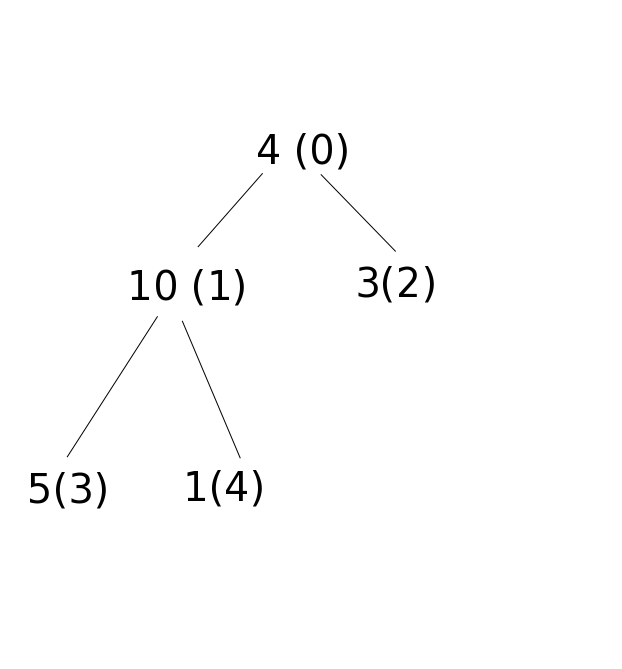
\includegraphics[height=3cm, width = 9cm]{./pic/g127-9.png}
			\caption{Exemplo de Heap}
		\end{figure}
	\end{block}
\end{frame}

\begin{frame}
	\begin{block}{Exemplo de heapficação}
		O processo de heapficação começa pelas folhas: $5,1,3$. 
		Em nenhum desses casos precisamos alterar a árvore.
		\begin{figure}[!htb]
			\centering	  				
			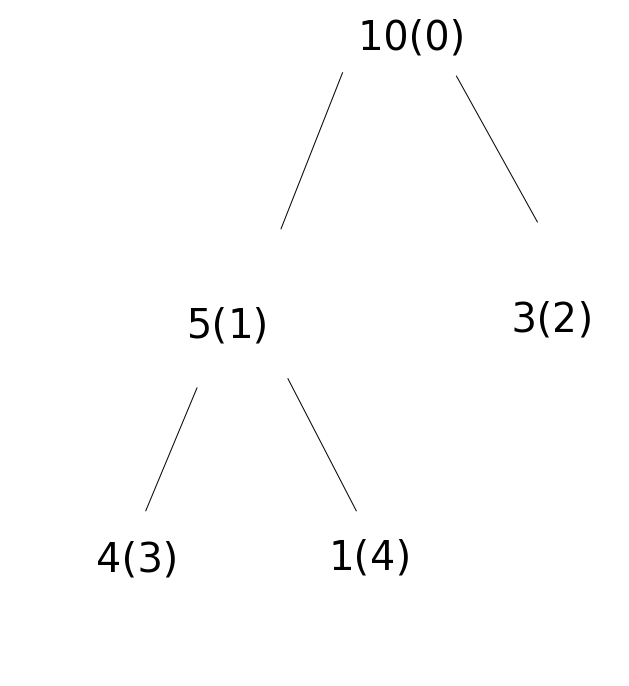
\includegraphics[height=3cm, width = 9cm]{./pic/g2755.png}
			\caption{Exemplo de Heap}
		\end{figure}
	\end{block}
\end{frame}


%\begin{frame}
%	\begin{block}{Exemplo de heapficação}
%		Ao aplicar a heapificação para a raiz percebemos que há necessidade de trocar valores.
%		\begin{figure}[!htb]
%			\centering	  				
%			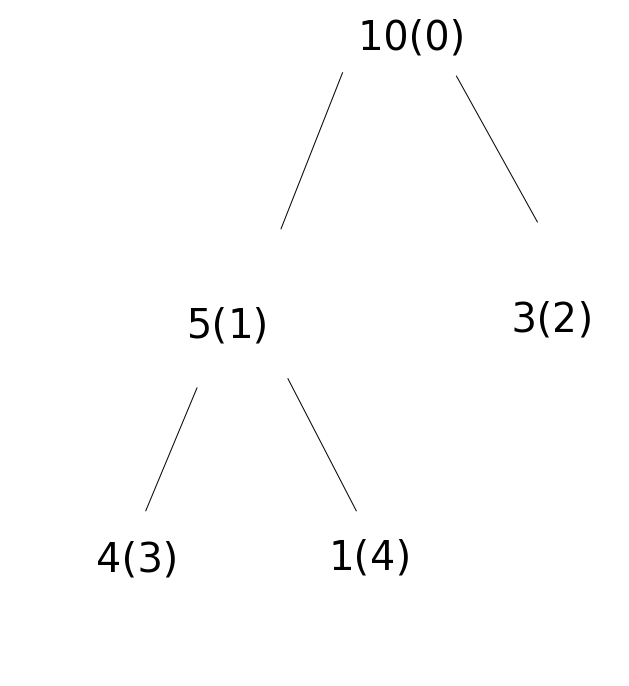
\includegraphics[height=3cm, width = 9cm]{./pic/g2755.png}
%			\caption{Exemplo de Heap}
%			\label{fig_pilha}
%		\end{figure}
%	\end{block}
%\end{frame}


\begin{frame}{}
	\begin{figure}[h!]
		\centering    
		\movie[
					   height = 6cm,%
		                width = 6cm,%
		                %poster,
		                showcontrols%
					] 
		  {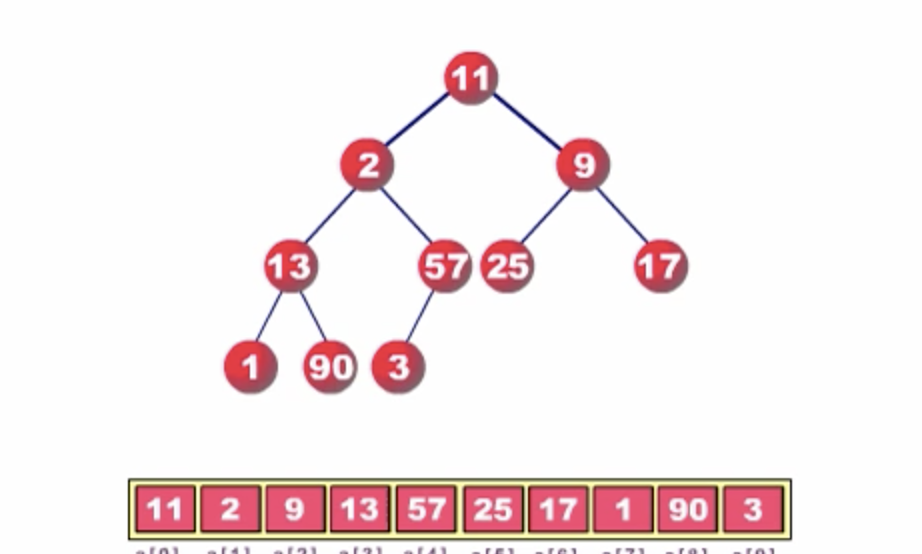
\includegraphics[width=5cm, height = 6cm]{./pic/heapImagePoster.png}}{./pic/heap-sort.mov}
		  \caption{Exemplo de ordenação com o Insertion Sort}
	 \end{figure} 
\end{frame}


\begin{frame}
	\begin{block}{Exemplo de uso do HeapSort}
		\begin{figure}[!htb]
			\centering	  				
			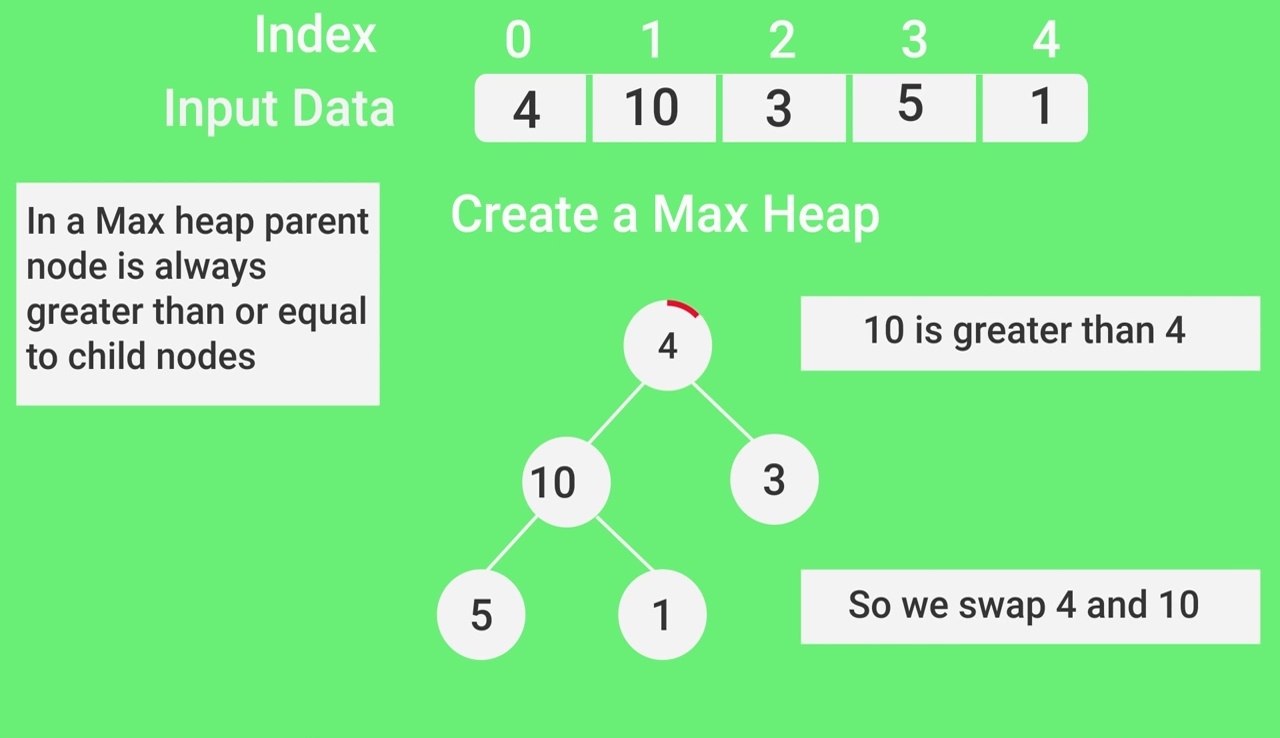
\includegraphics[height=3cm, width = 9cm]{./pic/scene01081.jpg}
			\caption{Exemplo de Heap}
		\end{figure}
	\end{block}
\end{frame}

\begin{frame}
	\begin{block}{Exemplo de uso do HeapSort}
		\begin{figure}[!htb]
			\centering	  				
			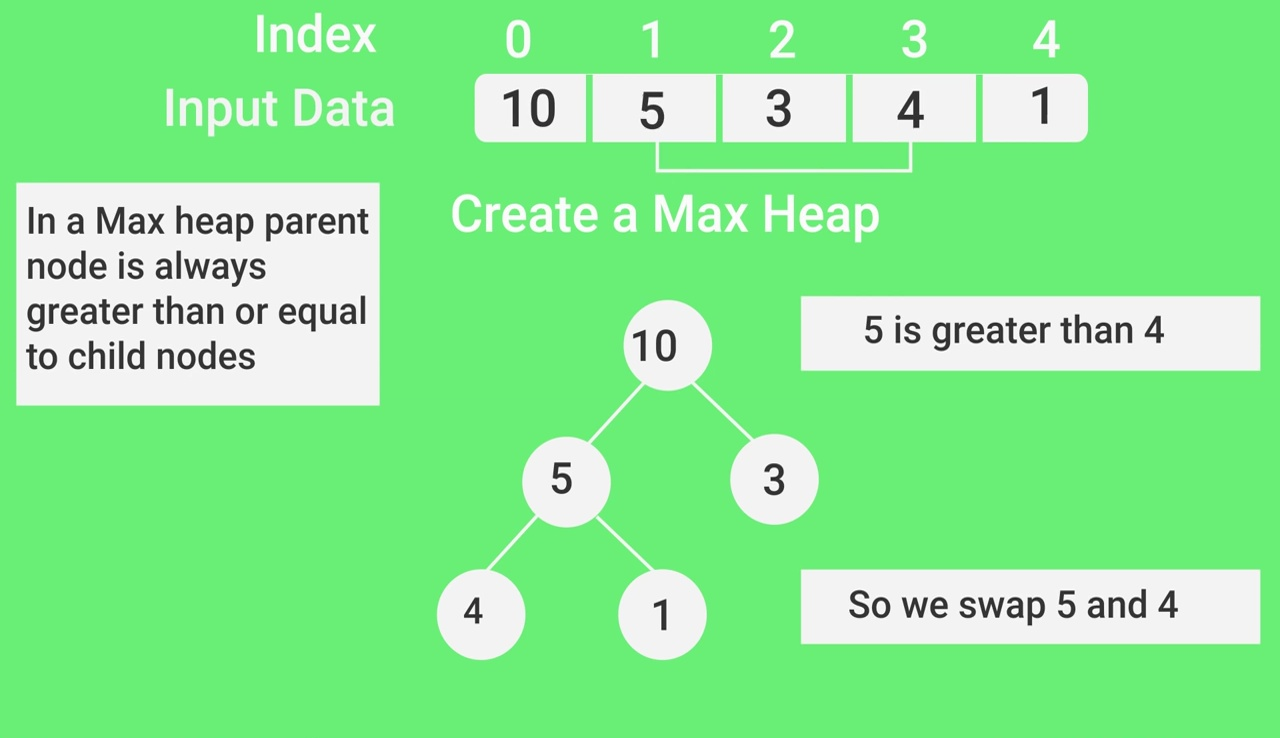
\includegraphics[height=3cm, width = 9cm]{./pic/scene01297.jpg}
			\caption{Exemplo de Heap}
		\end{figure}
	\end{block}
\end{frame}

\begin{frame}
	\begin{block}{Exemplo de uso do HeapSort}
		\begin{figure}[!htb]
			\centering	  				
			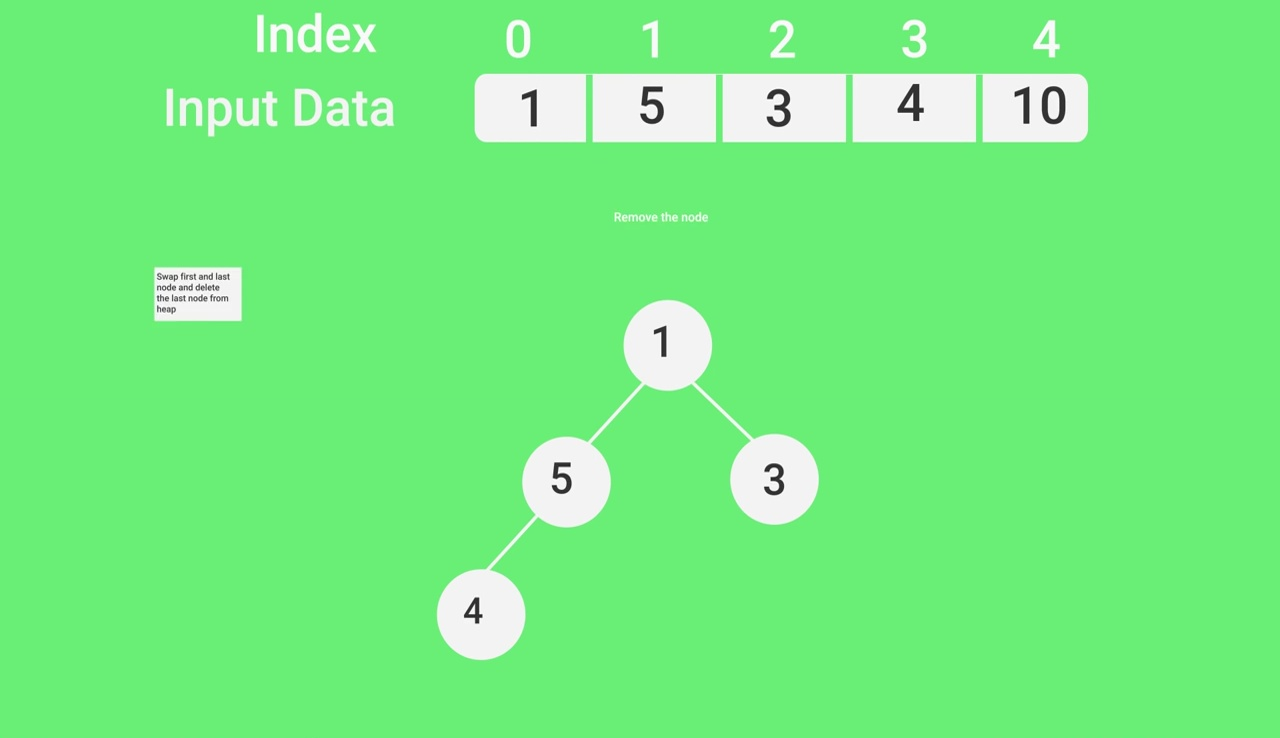
\includegraphics[height=3cm, width = 9cm]{./pic/scene01513.jpg}
			\caption{Exemplo de Heap}
		\end{figure}
	\end{block}
\end{frame}

\begin{frame}
	\begin{block}{Exemplo de uso do HeapSort}
		\begin{figure}[!htb]
			\centering	  				
			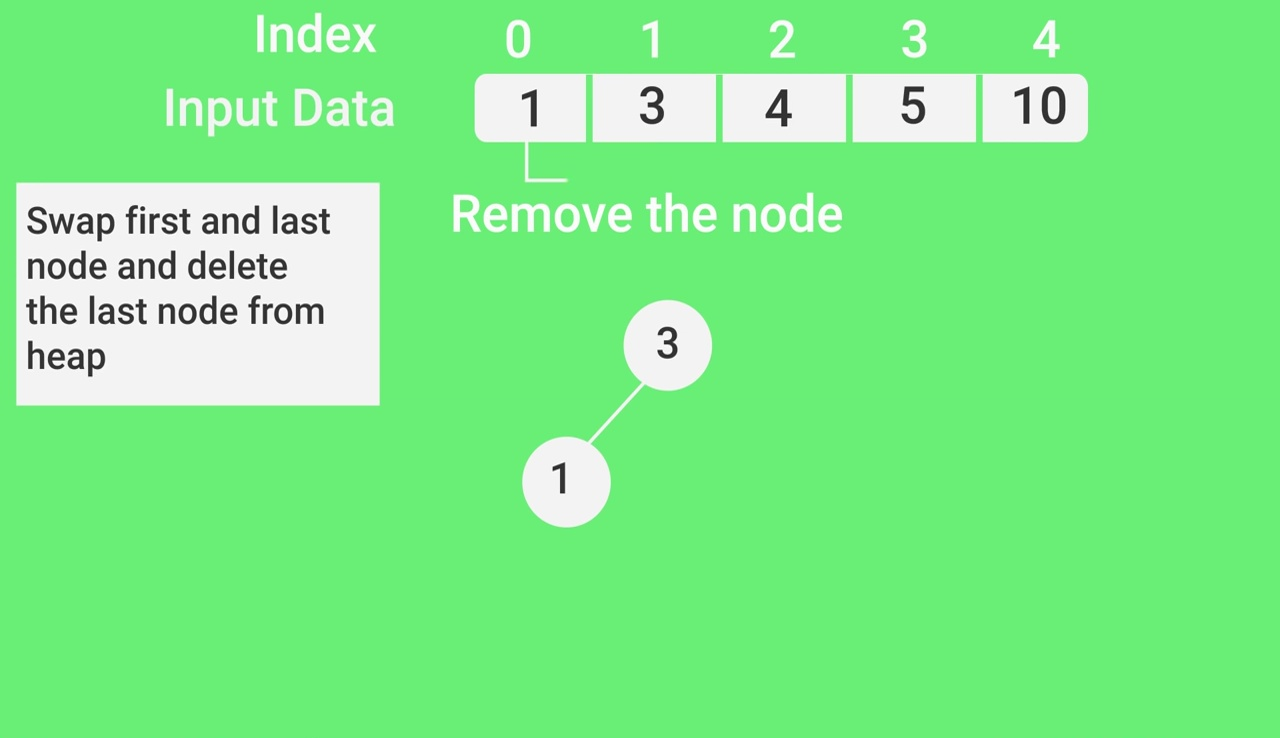
\includegraphics[height=3cm, width = 9cm]{./pic/scene02449.jpg}
			\caption{Exemplo de Heap}
		\end{figure}
	\end{block}
\end{frame}

\begin{frame}
	\begin{block}{Exemplo de uso do HeapSort}
		\begin{figure}[!htb]
			\centering	  				
			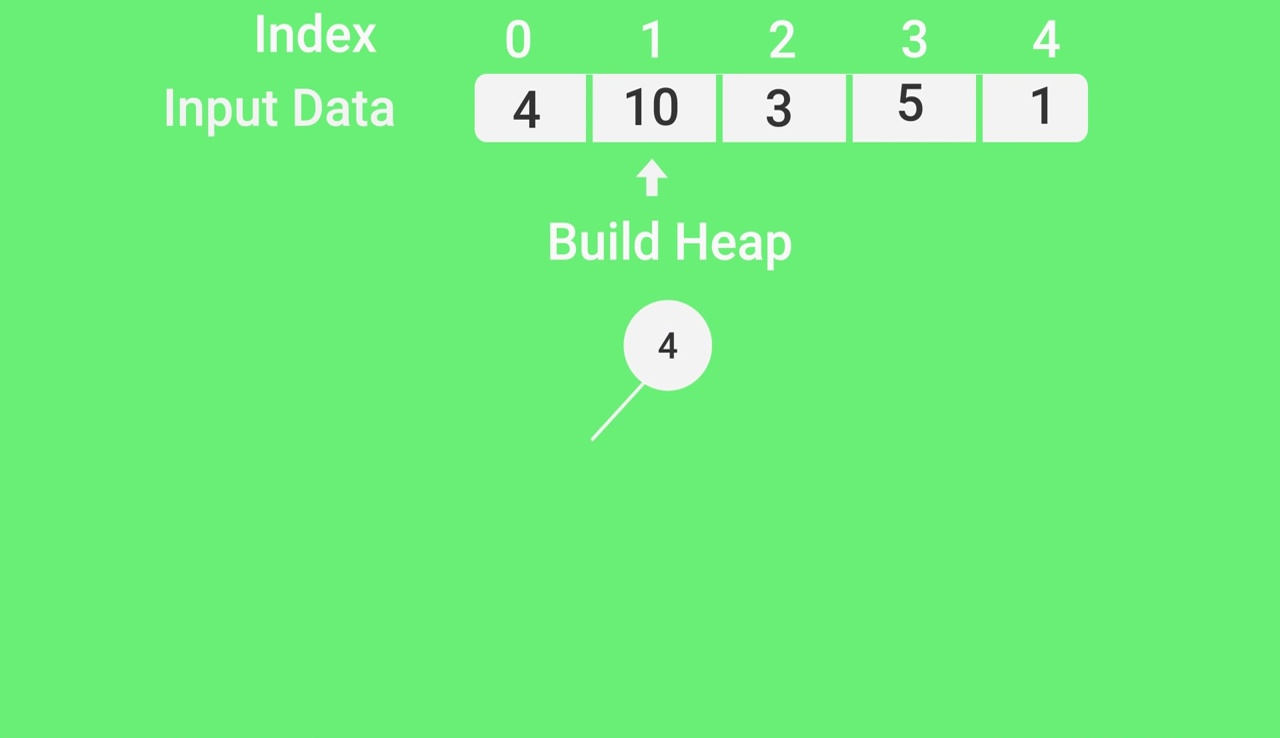
\includegraphics[height=3cm, width = 9cm]{./pic/scene005051.jpg}
			\caption{Exemplo de Heap}
		\end{figure}
	\end{block}
\end{frame}

\begin{frame}
	\begin{block}{Exemplo de uso do HeapSort}
		\begin{figure}[!htb]
			\centering	  				
			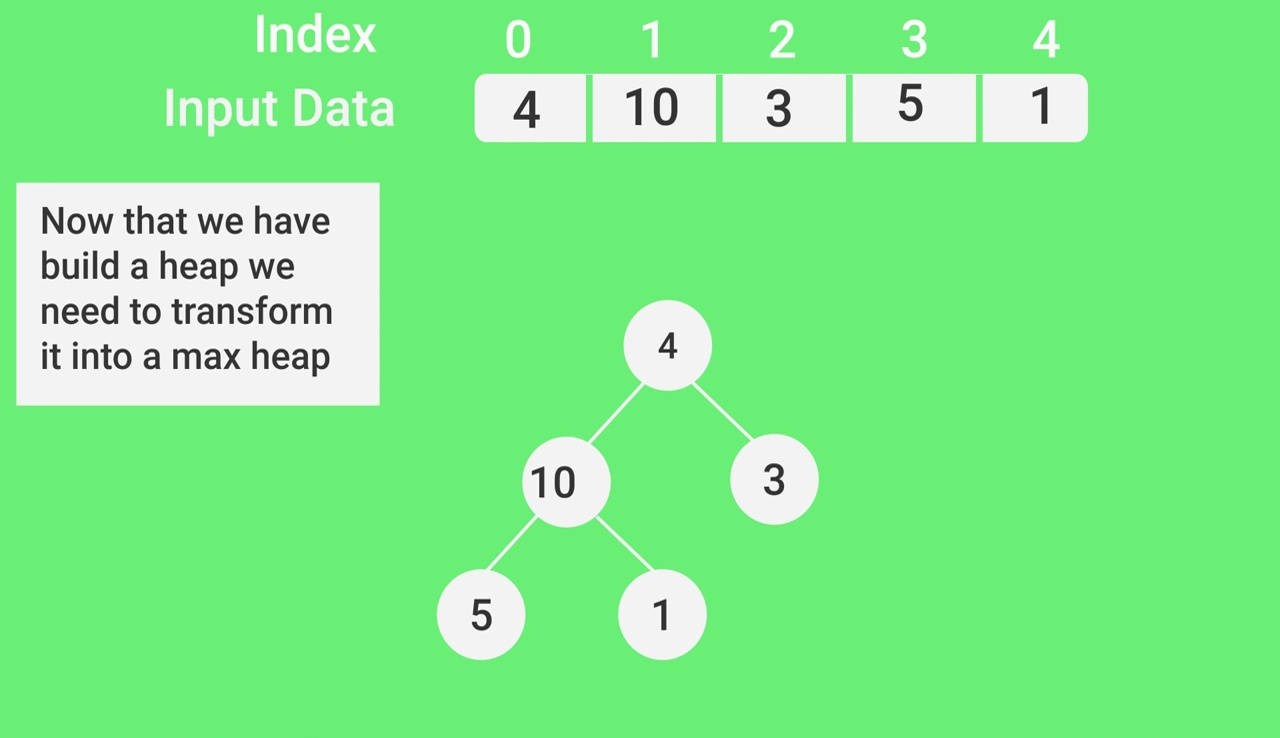
\includegraphics[height=3cm, width = 9cm]{./pic/scene007931.jpg}
			\caption{Exemplo de Heap}
		\end{figure}
	\end{block}
\end{frame}

\begin{frame}
	\begin{block}{Grafos}
		\begin{itemize}
			\item Programar com os alunos em C\#
			\item Discutir no quadro a comparação com outras estruturas
		\end{itemize}
	\end{block}
\end{frame}
